%% LyX 1.1 created this file.  For more info, see http://www.lyx.org/.
%% Do not edit unless you really know what you are doing.
\documentclass{article}
\usepackage[T1]{fontenc}
\usepackage{graphics}
\usepackage{longtable}

\makeatletter


%%%%%%%%%%%%%%%%%%%%%%%%%%%%%% LyX specific LaTeX commands.
\providecommand{\LyX}{L\kern-.1667em\lower.25em\hbox{Y}\kern-.125emX\@}
%% Special footnote code from the package 'stblftnt.sty'
%% Author: Robin Fairbairns -- Last revised Dec 13 1996
\let\SF@@footnote\footnote
\def\footnote{\ifx\protect\@typeset@protect
    \expandafter\SF@@footnote
  \else
    \expandafter\SF@gobble@opt
  \fi
}
\expandafter\def\csname SF@gobble@opt \endcsname{\@ifnextchar[%]
  \SF@gobble@twobracket
  \@gobble
}
\edef\SF@gobble@opt{\noexpand\protect
  \expandafter\noexpand\csname SF@gobble@opt \endcsname}
\def\SF@gobble@twobracket[#1]#2{}

%%%%%%%%%%%%%%%%%%%%%%%%%%%%%% Textclass specific LaTeX commands.
 \newcommand{\lyxaddress}[1]{
   \par {\raggedright #1 
   \vspace{1.4em}
   \noindent\par}
 }

\makeatother

\begin{document}


\title{\textbf{Linear scaling computation of the Fock matrix VI. Gaussian orbital
methods for DFT simulation of periodic systems}}


\author{C.J. Tymczak and Matt Challacombe}

\maketitle

\lyxaddress{Theoretical Division, Los Alamos National Laboratory, Los Alamos, New Mexico
87545}

\begin{abstract}
Periodic boundary conditions have been implemented in the linear scaling Quantum
Chemistry code \textbf{MondoSCF}. For the two-electron Coulomb matrix, this
has been achieved with an exact multipole expansion of the long range Coulomb
field. This yields a spherically summed boundary condition that is easily transformed
to Ewald boundary conditions. In order to achieve linear scaling of the local
Coulomb field, a Quantum Chemical Tree Code (QCTC) is used. Periodic boundary
conditions have also been incorporated into calculations of the local exchange-correlation
matrix. A Hierarchical Cubature (HiCu), pure Cartesian adaptive grid is used.
This method achieves linear scaling through the use of advanced data structures
(k-d trees) that maximally exploits locality of the density. Finally, the current
capabilities of MondoSCF for large condensed phases will be demonstrated.
\end{abstract}
\vfill\vfill\vfill \textbf{LA-UR-5555} \eject


\section{INTRODUCTION}

Periodic Boundary Conditions are often essential to employ when simulating bulk
behavior in solids or liquids. We have implemented Periodic boundary conditions
into the linear scaling Quantum Chemistry code \textbf{MondoSCF}. For the one
electron matrices this has been achieved by a re-summation over periodic cell
images, which because of locality leads to an efficient calculation of the one
electron integrals. For the two-electron Coulomb matrix, this has been achieved
with an exact multipole expansion of the long range Coulomb field. This yields
a spherically summed boundary condition that is easily transformed to Ewald
boundary conditions. In order to achieve linear scaling of the local Coulomb
field, a Quantum Chemical Tree Code (QCTC) is used. We have also incorporated
Periodic boundary conditions into calculations of the local exchange-correlation
matrix. A Hierarchical Cubature (HiCu), pure Cartesian adaptive grid is used.
This method achieves linear scaling through the use of advanced data structures
(k-d trees) that maximally exploits locality of the density, and allows for
an efficient treatment of the periodic effects. Next, we show the capabilities
of MondoSCF for three test condensed phases , Sodium Cloride, Magnesium Oxide
and Carbon in the Diamond and graphite structures. We then compare these results
to the periodic Gaussian code \textbf{Crystal98.} Next we demonstrate the utility
of the code on very large systems such as zeolite. Finally we give some conclusion
concerning the accuracy and utility of MondoSCF and future research directions.


\section{THEORY}


\subsection{One-Electron Matrices}


\subsubsection{The overlap matrix}

The first step in including periodic boundary conditions into our linear scaling
code is to determine the minimal modifications to the one-electron integrals
needed to obtain this. We incorporate periodic boundary conditions into our
linear scaling method by modifying the integrals. Consider the non-periodic
overlap matrix

\begin{equation}
\label{Sab_norm}
S_{ab}=\int _{V_{\infty }}\, d{\mathbf{x}}\, \phi _{a}({\mathbf{x}})\phi _{b}({\mathbf{x}})
\end{equation}
 where \( \{\phi _{a}(x),\phi _{b}(x)\} \) are the atomic orbitals (LCAO) at
atom \( a \) and atom \( b \) and \( V_{\infty } \) is the integration over
all space. In the periodic case this is replaced by,

\begin{equation}
\label{Sab_pbc1}
S_{ab}^{PBC}=\sum _{\mathbf{R},\mathbf{R}'}\int _{V_{cell}}\, d{\mathbf{x}}\, \phi _{a}({\mathbf{x}+R})\phi _{b}({\mathbf{x}+R'})
\end{equation}
where, \( V_{cell} \) is the integration over the simulation cell, and \( \{\mathbf{R},\mathbf{R}'\} \)
are the brava lattice vectors, this is illustrated in figure \ref{figure: SimCell},
where \( \left\{ {\mathbf{a},\mathbf{b},\mathbf{c}}\right\}  \) are the primitive
lattice vectors. Because of the locality of the atomic orbitals, we can remove
the double sum over lattice vectors to get

\begin{equation}
\label{Sab_pbc2}
S_{ab}^{PBC}=\sum _{\mathbf{R}}\int _{V_{\infty }}\, d{\mathbf{x}}\, \phi _{a}({\mathbf{x}})\phi _{b}({\mathbf{x}+R})
\end{equation}
We will use this Periodic Localization transformation (PL) repeatedly in what
follows. Let us also present some useful definitions:

\begin{equation}
\label{rho_loc}
\rho ^{loc}({\mathbf{x}})=\sum _{\mathbf{R}}\sum _{ab}{\mathbf{P}}_{ab}\phi _{a}({\mathbf{x}})\phi _{b}({\mathbf{x}+R})
\end{equation}
and because of periodicity,

\begin{equation}
\label{rho_pbc}
\rho ^{PBC}({\mathbf{x}})=\sum _{\mathbf{R}}\, \rho ^{loc}({\mathbf{x}+R})
\end{equation}
We also define:\begin{equation}
\label{rho_loc_ab}
\rho _{ab}^{loc}({\mathbf{x}})=\sum _{\mathbf{R}}\phi _{a}({\mathbf{x}})\phi _{b}({\mathbf{x}+R})
\end{equation}


\begin{equation}
\label{rho_pbc_ab}
\rho _{ab}^{PBC}({\mathbf{x}})=\sum _{R}\, \rho _{ab}^{loc}({\mathbf{x}+R})
\end{equation}
Which allows us to rewrite the overlap matrix matrix

\begin{equation}
\label{Sab_pbc_3}
S_{ab}^{PBC}=\int _{V_{\infty }}\, d{\mathbf{x}}\, \rho ^{loc}_{ab}({\mathbf{x}})
\end{equation}



\subsubsection{The Kinetic Energy Matrix}

The Kinetic energy matrix for the non-periodic case is given by

\begin{equation}
\label{Tab}
T_{ab}=-\frac{1}{2}\int _{V_{\infty }}\, d{\mathbf{x}}\, \phi _{a}({\mathbf{x}})\nabla ^{2}\phi _{b}({\mathbf{x}})
\end{equation}
Incorporating the PL transformation, we can rewrite this integral for the periodic
case as,\begin{equation}
\label{Tab_pbc}
T^{PBC}_{ab}=-\frac{1}{2}\sum _{\mathbf{R}}\int _{V_{\infty }}\, d{\mathbf{x}}\, \phi _{a}({\mathbf{x}+R})\nabla ^{2}\phi _{b}({\mathbf{x}})
\end{equation}



\subsection{The Two-Electron matrices}


\subsubsection{The Coulomb matrix}

We can transform the two-electron Coulomb integrals into integrals over all
space with local distributions via PL transformation and equations (\ref{rho_pbc})
and (\ref{rho_pbc_ab}), \begin{eqnarray}
J_{ab}^{PBC} & = & \frac{1}{2}\int _{V_{cell}}\int _{V_{\infty }}\, d{\mathbf{x}}\, d{\mathbf{x}'}\frac{\rho _{ab}^{PBC}\left( {\mathbf{x}}\right) \: \rho ^{PBC}\left( \mathbf{x}'\right) }{\left| \mathbf{x}-\mathbf{x}'\right| }\begin{array}{c}
\\

\end{array}\label{Jab_pbc1} \\
 & = & \frac{1}{2}\sum _{\mathbf{R}'}\int _{V_{\infty }}\int _{V_{\infty }}\, d{\mathbf{x}}\, d{\mathbf{x}'}\frac{\rho _{ab}^{loc}\left( {\mathbf{x}}\right) \: \rho ^{loc}\left( {\mathbf{x}'}+{\mathbf{R}'}\right) }{\left| \mathbf{x}-\mathbf{x}'\right| }\begin{array}{c}
\\

\end{array}\label{Jab_pbc2} 
\end{eqnarray}
let us separate the Coulomb integral into \[
J_{ab}^{PBC}=J_{ab}^{QCTC}+J_{ab}^{PFF}+J_{ab}^{EC}\]
where \begin{eqnarray}
J_{ab}^{QCTC} & = & \frac{1}{2}\sum _{{\mathbf{R}'}\in V_{in}}\, \int _{V_{\infty }}\, \int _{V_{\infty }}\, d{\mathbf{x}}\, d{\mathbf{x}'}\frac{\rho _{ab}^{loc}\left( {\mathbf{x}}\right) \: \rho ^{loc}\left( {\mathbf{x}'+\mathbf{R}'}\right) }{\left| \mathbf{x}-\mathbf{x}'\right| }\begin{array}{c}
\\

\end{array}\label{Jqctc} \\
J_{ab}^{PFF} & = & \frac{1}{2}\sum _{{\mathbf{R}'}\in V_{\infty }-V_{in}}\, \int _{V_{\infty }}\, \int _{V_{\infty }}\, d{\mathbf{x}}\, d{\mathbf{x}'}\frac{\rho _{ab}^{loc}\left( {\mathbf{x}}\right) \: \rho ^{loc}\left( {\mathbf{x}'+\mathbf{R}'}\right) }{\left| \mathbf{x}-\mathbf{x}'\right| }\begin{array}{c}
\\

\end{array}\label{Jpff} \\
J_{ab}^{EC} & = & \frac{1}{2}\sum _{{\mathbf{R}'}\in S_{\infty }}\, \int _{V_{\infty }}\, \int _{S_{\infty }}\, d{\mathbf{x}}\, d{\mathbf{x}'}\frac{\rho _{ab}^{loc}\left( {\mathbf{x}}\right) \: \rho ^{loc}\left( {\mathbf{x}'+\mathbf{R}'}\right) }{\left| \mathbf{x}-\mathbf{x}'\right| }\begin{array}{c}
\\

\end{array}\label{Jec} 
\end{eqnarray}
and \( V_{in} \) is the volume which contains the inner cells, \( V_{\infty } \)
is the total volume and \( S_{\infty } \) is the surface at infinity which
contributes a shape dependent potential to the center cell, which are depicted
in figure \ref{figure: ReplicateCells}. Let us now define each term.


\subsubsection{The Quantum Chemical Tree Code: The direct Coulomb matrix}

In-order to achieve linear scaling, we use a quantum chemical tree code {[}ref{]}
to compute the integral in equation (\ref{Jqctc}). This requires that we replace
the integrals in equation (\ref{Jqctc}) with the approximate spherical multipole
expansion to order \( L \) and \( L' \), \[
\frac{1}{2}\int _{V_{\infty }}\, d{\mathbf{x}}\, d{\mathbf{x}'}\frac{\rho _{ab}^{loc}\left( {\mathbf{x}}\right) \: \rho ^{loc}\left( {\mathbf{x}'}\right) }{\left| \mathbf{x}-\mathbf{x}'\right| }\approx \frac{1}{2}\sum _{\left\langle i\right\rangle }\int _{V_{\infty }}\, d{\mathbf{x}}\, d{\mathbf{x}'}\frac{\rho _{ab}^{loc}\left( {\mathbf{x}}\right) \: \Lambda ^{\left\langle i\right\rangle }\left( {\mathbf{x}'}\right) }{\left| \mathbf{x}-\mathbf{x}'\right| }\qquad \qquad \qquad \qquad \]
\begin{equation}
\label{QCTC}
+\frac{1}{2}\sum _{\left\langle j\neq i\right\rangle }\sum _{l=0}^{L}\, \sum _{l'=0}^{L'}\, \sum _{m=-l}^{l}\, \sum _{m'=-l'}^{l'}\, \left( -1\right) ^{l}\, \rho _{l}^{m}[{\mathbf{P}}]\, M_{l+l'}^{m+m'}[{\mathbf{P}-\mathbf{Q}}]\, \Lambda _{l'}^{\left\langle j\right\rangle ,m'}[{\mathbf{Q}}]\qquad 
\end{equation}
where

\begin{eqnarray}
\rho _{l}^{m}\left[ {\mathbf{P}}\right]  & = & \int _{V_{\infty }}\, d{\mathbf{x}}\, O_{l}^{m}\left[ {\mathbf{r}-\mathbf{P}}\right] \rho _{ab}^{loc}\left( {\mathbf{x}}\right) \begin{array}{c}
\\

\end{array}\label{sp_rho_ab} \\
\Lambda ^{\left\langle j\right\rangle ,m}_{l}\left[ {\mathbf{Q}}\right]  & = & \int _{V_{\infty }}\, d{\mathbf{x}}\, O_{l}^{m}\left[ {\mathbf{r}-\mathbf{Q}}\right] \Lambda ^{\left\langle j\right\rangle }\left( {\mathbf{x}}\right) \begin{array}{c}
\\

\end{array}\label{sp_rho_loc} 
\end{eqnarray}
and

\begin{eqnarray}
O_{l}^{m}\left[ {\mathbf{R}}\right]  & = & \frac{\left| {\mathbf{R}}\right| ^{l}P_{l}^{m}\left( \cos \left( \theta _{\mathbf{R}}\right) \right) \, e^{-im\phi _{\mathbf{R}}}}{\left( l+m\right) !}\begin{array}{c}
\\

\end{array}\label{sp_mult_O} \\
M_{l}^{m}\left[ {\mathbf{R}}\right]  & = & \frac{\left( l-m\right) !\, P_{l}^{m}\left( \cos \left( \theta _{\mathbf{R}}\right) \right) \, e^{-im\phi _{\mathbf{R}}}}{\left| {\mathbf{R}}\right| ^{l+1}}\begin{array}{c}
\\

\end{array}\label{sp_mult_M} 
\end{eqnarray}
and \( \left\langle i\right\rangle  \) and \( \left\langle j\neq i\right\rangle  \)
are the sums over distributions determined from the density tree. In reference
{[}ref{]} we give a derivation of the exact error bound we use to compute these
integrals in the QCTC algorithm which leads to excellent control over the error.

The Periodic Far Field Coulomb matrix

To obtain the periodic far field correction to the matrix elements we replace
the integral in equation (\ref{Jpff}) with the multipole sum

\begin{eqnarray}
J_{ab}^{PFF} & = & \frac{1}{2}\sum _{{\mathbf{R}'}\in V_{\infty }-V_{in}}\, \int _{V_{\infty }}\, d{\mathbf{x}}\, d{\mathbf{x}'}\frac{\rho _{ab}^{loc}\left( {\mathbf{x}}\right) \: \rho ^{loc}\left( {\mathbf{x}'+\mathbf{R}'}\right) }{\left| \mathbf{x}-\mathbf{x}'\right| }\begin{array}{c}
\\

\end{array}\label{jpff_2} \\
 & = & \frac{1}{2}\sum _{{\mathbf{R}'}\in V_{\infty }-V_{in}}\, \sum _{l=0}^{L}\, \sum _{l'=0}^{L'}\, \sum _{m=-l}^{l}\, \sum _{m'=-l'}^{l'}\, \left( -1\right) ^{l}\, \rho _{l}^{m}[{\mathbf{P}}]\, M_{l+l'}^{m+m'}[{\mathbf{P}-\mathbf{Q}}]\, \rho _{l'}^{m'}[{\mathbf{Q}+\mathbf{R}'}]\begin{array}{c}
\\

\end{array}\label{sp_jpff} 
\end{eqnarray}
which setting \( P=R_{0} \) and \( Q=R_{0}-R' \) we can rewrite as\begin{equation}
\label{sp_jpff_2}
J_{ab}^{PFF}=\frac{1}{2}\sum _{l=0}^{L}\, \sum _{l'=0}^{L'}\, \sum _{m=-l}^{l}\, \sum _{m'=-l'}^{l'}\, \left( -1\right) ^{l}\, \rho _{l}^{m}[{\mathbf{R}_{0}}]\, {\cal M}_{l+l'}^{m+m'}\, \rho _{l'}^{m'}[{\mathbf{R}_{0}}]
\end{equation}
where

<empty clipboard>\begin{equation}
\label{ScriptM}
{\cal M}_{l}^{m}=\sum _{{\mathbf{R}'}\in V_{\infty }-V_{in}}\, M_{l}^{m}[\mathbf{R}]
\end{equation}
which for \( l<3 \) is a conditional summation. In appendix A we describe an
efficient method which allow us calculate these conditional summations. In the
next section we describe the corrections to the Coulomb matrix which allow us
to obtain Ewald boundary conditions so that we can compare directly to \textbf{Crystal98}.
Figure \ref{figure: ErrorPFF} shows the error of the energy as we increase
the Inner box sums for \( L=8,16 \) for a sodium cloride test system, as can
be seen we obtain very rapid convergence.


\subsubsection{The Ewald Correction matrix}

The correction to the Coulomb matrix is strongly dependent on how the periodic
multipole tensor is summed. If the matrix is a spherically ordered lattice sum,
then the connection between the spherically ordered potential and the Ewald
potential is {[}ref{]}, \begin{equation}
\label{EW_pot}
\Phi _{Ew}\left( \mathbf{x}\right) =\Phi _{ss}\left( \mathbf{x}\right) -\frac{4\pi }{3}{\left( \mathbf{x}-\mathbf{R}_{0}\right) \cdot \mathbf{D}}+\frac{2\pi }{3}Q
\end{equation}
in terms of the matrix elements of \( J_{ab}^{PBC} \) this gives the corrections\begin{eqnarray}
J_{ab}^{EC} & = & \int _{V_{\infty }}\, d{\mathbf{x}}\, \rho ^{loc}_{ab}\left( {\mathbf{x}}\right) \left\{ \frac{2\pi }{3}Q-\frac{4\pi }{3}\left( \mathbf{x}-\mathbf{R}_{0}\right) \cdot \mathbf{D}\right\} \begin{array}{c}
\\

\end{array}\label{Jab_ec} \\
 & = & \frac{2\pi }{3}Q\, S_{ab}^{PBC}-\frac{4\pi }{3}\mathbf{d}_{ab}\cdot \mathbf{D}\label{Jab_ec_2} 
\end{eqnarray}
where

\begin{eqnarray}
{\mathbf{d}}_{ab} & = & \int _{V_{\infty }}\, d{\mathbf{x}}\, \left( \mathbf{x}-\mathbf{R}_{0}\right) \rho ^{loc}_{ab}\left( \mathbf{x}\right) \begin{array}{c}
\\

\end{array}\label{dab} \\
{\mathbf{D}} & = & \int _{V_{\infty }}\, d{\mathbf{x}}\, \left( \mathbf{x}-\mathbf{R}_{0}\right) \rho ^{loc}\left( \mathbf{x}\right) \begin{array}{c}
\\

\end{array}\label{D} \\
Q & = & \int _{V_{\infty }}\, d{\mathbf{x}}\, \left( \mathbf{x}-\mathbf{R}_{0}\right) ^{2}\rho ^{loc}\left( \mathbf{x}\right) \begin{array}{c}
\\

\end{array}\label{Q} 
\end{eqnarray}
are the dipole and quadrapole moments. In appendix 


\subsubsection{The exchange correlation matrix}

To calculate the exchange correlation matrix in the periodic case, we take advantage
of the periodicity of the functions being integrated and the locality of the
basis functions,

\begin{eqnarray}
K_{ab}^{PBC} & = & \int _{V_{cell}}\, d\mathbf{x}\, \rho _{ab}^{PBC}\left( \mathbf{x}\right) \: V_{xc}\left( \rho ^{PBC}\left( \mathbf{x}\right) \right) \begin{array}{c}
\\

\end{array}\label{Kab_pbc_1} \\
 & = & \int _{V_{HiCu}}\, d\mathbf{x}\, \rho _{ab}^{PBC}\left( \mathbf{x}\right) \: V_{xc}\left( \rho ^{PBC}\left( \mathbf{x}\right) \right) \begin{array}{c}
\\

\end{array}\label{Kab_pbc_2} \\
 & = & \sum _{RR'}\int _{V_{HiCu}}\, d\mathbf{x}\, \phi _{a}(\mathbf{x}+R)\phi _{b}(\mathbf{x}+R')\, V_{xc}\left( \sum _{R''}\, \rho ^{loc}\left( \mathbf{x}+R''\right) \right) \begin{array}{c}
\\

\end{array}\label{Kab_pbc_3} 
\end{eqnarray}
where \( V_{HiCu} \) is the cubic region shown in figure \ref{figure: SimCell}.
This transformation is allowable because of the periodicity of the function,
and it is ideally suited for the method we use to calculate our exchange-correlation
matrix, which is based on a {}``Gaussian quadrature{}'' integration of a rectangular
region. To calculate the exchange correlation matrix in periodic system we need
to use equation (\ref{Kab_pbc_3}). This could be prohibitively expensive because
of the double sum if not for the locality of the HiCu grid. We have determined
that the the computational cost increases by about a factor of two. This is
achieved by splitting the problem into two steps

\begin{itemize}
\item First, we calculate the exchange-correlation potential on the HiCu grid using
the periodically summed local density \( \rho ^{loc}\left( \mathbf{x}\right)  \),
because of the k-d tree structure of the density this is not computationally
expensive.
\item Next, we directly calculate the integral of equation (\ref{Kab_pbc_3}), where
we obtain significant increase in efficacy by exploiting the localization of
the atomic orbitals. 
\end{itemize}

\section{RESULTS}


\subsection{Verification}

Table \ref{table:ComToCrystal98_1}-\ref{table:ComToCrystal98_3} displays our
results for several test systems, Sodium Cloride, Magnesium oxide , Diamond
and Graphite. We chose these systems because they are well studied and form
a distributions of the many bounding mechanisms which are possible, from Ionic
to covallent {[}ref{]}.


\subsubsection{Sodium Cloride}

Table \ref{table:ComToCrystal98_1} shows our results for the total energy for
Sodium Cloride as compared to results obtained from \textbf{Crystal98}. We test
this system in two different cell geometries, one cubic and the other orthorombic.
Also we use three different basis sets STO-3G, 3-21G and 6-31G{*}{*}. We only
use the Slater-Dirac functional because of convergence issues with \textbf{Crystal98}.
We obtain excellent agreement with \textbf{Crystal98} to the accuracy of there
results, however, \textbf{MondoSCF} is capable of obtaining very precise results,
beyond the capacity of \textbf{Crystal98} because we do not use fitting functions
in the calculations of the Coulomb or the exchange-correlation energies. 


\subsubsection{Magnesium Oxide}

Table \ref{table:ComToCrystal98_2} shows our results for the total energy for
Magnesium Oxide as compared to results obtained from \textbf{Crystal98}. Because
of the high degree of Ionic bounding in this system, \textbf{Crystal98} does
substantially better then for sodium Cloride. This allows for a much closer
scrutiny of the energies then for the previous system. Again, we obtain excellent
agreement with \textbf{Crystal98} for three different basis sets to within the
accuracy of these results.


\subsubsection{Diamond and Graphite}

Table \ref{table:ComToCrystal98_3} shows our results for the total energy for
Diamond and Graphite as compared to results obtained from \textbf{Crystal98}.


\subsection{Scaling}

For testing of linear scaling, we us a set of dense molecular nitrogen systems
obtained from molecular dynamics simulations. Figure \ref{figure:DenseNitrogen}
shows a Iso-surface potential plot for the largest test system, a dense gas
of 100 \( N_{2} \) nitrogen molecules. The electronic iso-surface is at a density
of 0.4, and the colors represent the Coulomb potential projected upon this surface,
yellow being positive and blue being negative. Figure \ref{figure: Scaling_Matrix_Build}
shows our scaling results of the dense nitrogen periodic system for both the
\( J_{QCTC} \) and \( K_{xc} \) matrix builds for two different error thresholds.
Figure \ref{figure:Scaling_Diag} also shows scaling results, for these same
system and thresholds, for the overlap matrix inverter and the density matrix
calculator. Even in this dense periodic system, linear scaling commences very
early, around twenty molecules. Also, we mention the fact that the crossover
for linear scaling for the density matrix solver, as opposed to the eigen-solver,
is around 50 molecules even for these small basis set systems. 


\subsection{Zeolite}


\section{CONCLUSIONS}

Periodic Boundary Conditions are often essential to employ when simulating bulk
behavior in solids or liquids. We have implemented Periodic boundary conditions
into the linear scaling Quantum Chemistry code \textbf{MondoSCF}. For the one
electron matrices this has been achieved by a re-summation over periodic cell
images, which because of locality leads to an efficient calculation of the one
electron integrals. For the two-electron Coulomb matrix, this has been achieved
with an exact multipole expansion of the long range Coulomb field. This yields
a spherically summed boundary condition that is easily transformed to Ewald
boundary conditions. In order to achieve linear scaling of the local Coulomb
field, a Quantum Chemical Tree Code (QCTC) is used. We have also incorporated
Periodic boundary conditions into calculations of the local exchange-correlation
matrix. A Hierarchical Cubature (HiCu), pure Cartesian adaptive grid is used.
This method achieves linear scaling through the use of advanced data structures
(k-d trees) that maximally exploits locality of the density, and allows for
an efficient treatment of the periodic effects. Next, we show the capabilities
of MondoSCF for three test condensed phases , Sodium Cloride, Magnesium Oxide
and Carbon in the Diamond and graphite structures. We then compare these results
to the periodic Gaussian code \textbf{Crystal98.} Next we demonstrate the utility
of the code on very large systems such as zeolite. Finally we give some conclusion
concerning the accuracy and utility of MondoSCF and future research directions.


\section*{ACKNOWLEDGMENTS}

We would like to acknowledge Tommy Sewell and Ed Kober for there advise and
support. \eject

\appendix

\section*{Computation of the \protect\( {\cal M}\protect \) Tensor}

Following the work of Nijboer-De Wette et.al. We start by first partitioning
 

\begin{equation}
\frac{1}{r^{l+1}}={\cal G}_{l}\left( \beta ,r\right) +{\cal F}_{l}\left( \beta ,r\right) 
\end{equation}
where

\begin{equation}
{\cal G}_{l}\left( \beta ,r\right) =\frac{\Gamma \left( l+\frac{1}{2},\beta ^{2}r^{2}\right) }{\Gamma \left( l+\frac{1}{2}\right) \, r^{l+1}}
\end{equation}
and\begin{equation}
{\cal F}_{l}\left( \beta ,r\right) =\frac{\gamma \left( l+\frac{1}{2},\beta ^{2}r^{2}\right) }{\Gamma \left( l+\frac{1}{2}\right) \, r^{l+1}}=\frac{\Gamma \left( l+\frac{1}{2}\right) -\Gamma \left( l+\frac{1}{2},\beta ^{2}r^{2}\right) }{\Gamma \left( l+\frac{1}{2}\right) \, r^{l+1}}
\end{equation}
where \( \beta  \) is a parameter which controls the convergence. This allows
the lattice sum to be partitioned into rapidly convergent real and reciprocal
space terms 

\begin{eqnarray}
{\cal M}^{m}_{l} & = & \sum _{{\mathbf{R}'}\in V_{\infty }-V_{in}}\, M_{l}^{m}[\mathbf{R}]\begin{array}{c}
\\

\end{array}\nonumber \\
 & = & \sum _{{\mathbf{R}'}\in V_{\infty }-V_{in}}\, \left( l-m\right) !\, P_{l}^{m}\left( \cos \left( \theta _{\mathbf{R}}\right) \right) e^{im\phi _{\mathbf{R}}}\, \left\{ {\cal G}_{l}\left( \beta ,\left| \mathbf{R}\right| \right) +{\cal F}_{l}\left( \beta ,\left| \mathbf{R}\right| \right) \right\} \begin{array}{c}
\\

\end{array}\nonumber \\
 & = & \sum _{{\mathbf{R}'}\in V_{\infty }-V_{in}}\, \left( l-m\right) !\, P_{l}^{m}\left( \cos \left( \theta _{\mathbf{R}}\right) \right) e^{im\phi _{\mathbf{R}}}\, {\cal G}_{l}\left( \beta ,\left| \mathbf{R}\right| \right) \begin{array}{c}
\\

\end{array}\nonumber \\
 & - & \sum _{{\mathbf{R}'}\in V_{in}}\, \left( l-m\right) !\, P_{l}^{m}\left( \cos \left( \theta _{\mathbf{R}}\right) \right) e^{im\phi _{\mathbf{R}}}{\cal F}_{l}\left( \beta ,\left| \mathbf{R}\right| \right) \begin{array}{c}
\\

\end{array}\nonumber \\
 & + & \frac{4\pi ^{\frac{3}{2}}(\frac{i}{2})^{l}}{\Gamma \left( l+\frac{1}{2}\right) }\sum _{\mathbf{G}\neq \left\{ \emptyset \right\} }\, \left| \mathbf{G}\right| ^{l-2}e^{-\frac{\pi ^{2}\left| \mathbf{G}\right| ^{2}}{\beta ^{2}}}\, \left( l-m\right) !\, P_{l}^{m}\left( \cos \left( \theta _{\mathbf{G}}\right) \right) e^{im\phi _{\mathbf{G}}}
\end{eqnarray}
With an appropriate choice of \( \beta \sim \sqrt{\pi }/V^{\frac{1}{3}} \)
the periodic multipole interaction tensor can be computed. The only potential
problem is the computation of the incomplete gamma functions. Previous approaches
attempted to compute this function by the upward recurrence relation

\begin{equation}
\Gamma \left( m+1,\, x\right) =m\Gamma \left( m,\, x\right) +x^{m}e^{-x}
\end{equation}
which is started by

\begin{equation}
\label{erfc}
\Gamma \left( \frac{1}{2},\, x\right) =\sqrt{\pi }\, {\rm erfc}\left( \sqrt{x}\right) 
\end{equation}
however, this leads a numerical instability in the calculation. For large values
of \( x \) and \( m \) the calculation of the gamma function can quickly lose
precision. We can remove this problem by analytically summing the gamma function,
collecting terms, and then rewriting the gamma function as\begin{equation}
\Gamma \left( m+\frac{1}{2},\, x\right) =\Gamma \left( m+\frac{1}{2}\right) \left\{ {\rm erfc}\left( \sqrt{x}\right) +\sqrt{\frac{x}{\pi }}\sum _{n=0}^{m-1}(S_{n}\, x\, e^{-\frac{x}{n}})^{n}\right\} 
\end{equation}
where

\begin{equation}
\label{SN}
S_{n}=\left( \frac{\Gamma \left( \frac{1}{2}\right) }{\Gamma \left( n+\frac{3}{2}\right) }\right) ^{\frac{1}{max(n,1)}}
\end{equation}
Which are tabulated beforehand. We find that this version of the gamma function
is both easy to program and numerically very precise, even at large \( x \)
or \( m \). Table \ref{table:CubicMlm} shows the matrix coefficients calculated
for different cell shapes. 


\section*{Computation of the Dipole and Quadrapole Corrections }

Following the work of Grindley et. al. \begin{equation}
\label{BN}
S_{n}=\left( \frac{\Gamma \left( \frac{1}{2}\right) }{\Gamma \left( n+\frac{1}{2}\right) }\right) ^{\frac{1}{n}}
\end{equation}
\eject


\section*{\bibliographystyle{plain}
\bibliography{gaussian}
}

\eject


\begin{table}

\caption{\label{table:ComToCrystal98_1}Comparison of Sodium Cloride test systems to
Crystal98}
{\centering \begin{tabular}{|c|c|c|c|c|c|}
\hline 
System&
Basis&
Functional&
Cell (A)&
Program&
Energy (Hartree)\\
\hline 
\hline 
NaCl&
STO-3G&
Slater-Dirac&
\( \left\{ \begin{array}{c}
\left| a\right| =\left| b\right| =\left| c\right| =3.974\\
\alpha =\frac{\pi }{3},\beta =\frac{\pi }{3},N=2
\end{array}\right\}  \)&
MondoSCF&
\( -610.9751176 \)\\
\hline 
&
&
&
\( \begin{array}{c}
\\

\end{array} \)&
Crystal98&
\( -610.972 \)\\
\hline 
&
STO-6G&
Slater-Dirac&
\( \begin{array}{c}
\\

\end{array} \)&
MondoSCF&
\\
\hline 
&
&
&
\( \begin{array}{c}
\\

\end{array} \)&
Crystal98&
\\
\hline 
&
STO-3G{*}{*}&
Slater-Dirac&
\( \begin{array}{c}
\\

\end{array} \)&
MondoSCF&
\\
\hline 
&
&
&
\( \begin{array}{c}
\\

\end{array} \)&
Crystal98&
\\
\hline 
\hline 
NaCl&
STO-3G&
Slater-Dirac&
\( \left\{ \begin{array}{c}
\left| a\right| =\left| b\right| =\left| c\right| =5.63\\
\alpha =\frac{\pi }{2},\beta =\frac{\pi }{2},N=8
\end{array}\right\}  \)&
MondoSCF&
\( -2444.3583560 \)\\
\hline 
&
&
&
\( \begin{array}{c}
\\

\end{array} \)&
Crystal98&
\( -2444.358 \)\\
\hline 
&
STO-6G&
Slater-Dirac&
\( \begin{array}{c}
\\

\end{array} \)&
MondoSCF&
\\
\hline 
&
&
&
\( \begin{array}{c}
\\

\end{array} \)&
Crystal98&
\\
\hline 
&
STO-3G{*}{*}&
Slater-Dirac&
\( \begin{array}{c}
\\

\end{array} \)&
MondoSCF&
\\
\hline 
&
&
&
\( \begin{array}{c}
\\

\end{array} \)&
Crystal98&
\\
\hline 
\end{tabular}\par}\vspace{0.3cm}
\end{table}

\begin{table}

\caption{\label{table:ComToCrystal98_2}Comparison of MgO test systems to Crystal98}
{\centering \begin{tabular}{|c|c|c|c|c|c|}
\hline 
System&
Basis&
Functional&
Cell (A)&
Program&
Energy (Hartree)\\
\hline 
\hline 
MgO&
STO-3G&
Slater-Dirac&
\( \left\{ \begin{array}{c}
\left| a\right| =\left| b\right| =\left| c\right| =2.9777\\
\alpha =\frac{\pi }{3},\beta =\frac{\pi }{3},N=2
\end{array}\right\}  \)&
MondoSCF&
\( -268.6324824 \)\\
\hline 
&
&
&
\( \begin{array}{c}
\\

\end{array} \)&
Crystal98&
\( -268.6323 \)\\
\hline 
&
STO-6G&
Slater-Dirac&
\( \begin{array}{c}
\\

\end{array} \)&
MondoSCF&
\( -269.384298 \)9\\
\hline 
&
&
&
\( \begin{array}{c}
\\

\end{array} \)&
Crystal98&
\\
\hline 
&
STO-3G{*}{*}&
Slater-Dirac&
\( \begin{array}{c}
\\

\end{array} \)&
MondoSCF&
\\
\hline 
&
&
&
\( \begin{array}{c}
\\

\end{array} \)&
Crystal98&
\\
\hline 
\hline 
MgO&
STO-3G&
Slater-Dirac&
\( \left\{ \begin{array}{c}
\left| a\right| =\left| b\right| =\left| c\right| =4.2112\\
\alpha =\frac{\pi }{3},\beta =\frac{\pi }{3},N=2
\end{array}\right\}  \)&
MondoSCF&
\( -1076.2137742 \)\\
\hline 
&
&
&
\( \begin{array}{c}
\\

\end{array} \)&
Crystal98&
\( -1076.2138 \)\\
\hline 
&
STO-6G&
Slater-Dirac&
\( \begin{array}{c}
\\

\end{array} \)&
MondoSCF&
\\
\hline 
&
&
&
\( \begin{array}{c}
\\

\end{array} \)&
Crystal98&
\\
\hline 
&
STO-3G{*}{*}&
Slater-Dirac&
\( \begin{array}{c}
\\

\end{array} \)&
MondoSCF&
\\
\hline 
&
&
&
\( \begin{array}{c}
\\

\end{array} \)&
Crystal98&
\\
\hline 
\end{tabular}\par}\end{table}



\begin{table}

\caption{\label{table:ComToCrystal98_3}Comparison of Carbon test systems to Crystal98}
{\centering \begin{tabular}{|c|c|c|c|c|c|}
\hline 
System&
Basis&
Functional&
Cell (A)&
Program&
Energy (Hartree)\\
\hline 
\hline 
Diamond&
STO-3G&
Slater-Dirac&
\( \left\{ \begin{array}{c}
\left| a\right| =\left| b\right| =\left| c\right| =\\
\alpha =\frac{\pi }{2},\beta =\frac{\pi }{2},N=8
\end{array}\right\}  \)&
MondoSCF&
\\
\hline 
&
&
&
\( \begin{array}{c}
\\

\end{array} \)&
Crystal98&
\\
\hline 
&
STO-6G&
Slater-Dirac&
\( \begin{array}{c}
\\

\end{array} \)&
MondoSCF&
\\
\hline 
&
&
&
\( \begin{array}{c}
\\

\end{array} \)&
Crystal98&
\\
\hline 
&
3-21G&
Slater-Dirac&
\( \begin{array}{c}
\\

\end{array} \)&
MondoSCF&
\\
\hline 
&
&
&
\( \begin{array}{c}
\\

\end{array} \)&
Crystal98&
\\
\hline 
\hline 
Graphite&
STO-3G&
Slater-Dirac&
\( \left\{ \begin{array}{c}
\left| a\right| =\left| b\right| =\left| c\right| =\\
\alpha =\frac{\pi }{2},\beta =\frac{\pi }{2},N=6
\end{array}\right\}  \)&
MondoSCF&
\\
\hline 
&
&
&
\( \begin{array}{c}
\\

\end{array} \)&
Crystal98&
\\
\hline 
&
3-21G&
Slater-Dirac&
\( \begin{array}{c}
\\

\end{array} \)&
MondoSCF&
\\
\hline 
&
&
&
\( \begin{array}{c}
\\

\end{array} \)&
Crystal98&
\\
\hline 
&
6-31G{*}{*}&
Slater-Dirac&
\( \begin{array}{c}
\\

\end{array} \)&
MondoSCF&
\\
\hline 
&
&
&
\( \begin{array}{c}
\\

\end{array} \)&
Crystal98&
\\
\hline 
\end{tabular}\par}\end{table}

\begin{table}

\caption{\label{table: ConvegOfNaCl} Total energy per atom for the sodium cloride system
for increasing system size}
{\centering \begin{tabular}{|c|c|c|}
\hline 
System Size (\( N) \)&
Energy (\( E \))&
\( \frac{E}{N} \)\\
\hline 
\hline 
\( \, \, 2^{\dagger } \)&
\( -610.975117 \)&
\( -305.487559 \)\\
\hline 
\( 8 \)&
\( -2444.35835 \)&
\( -305.544794 \)\\
\hline 
\( \, \, 16^{\dagger } \)&
\( -4888.70023 \)&
\( -305.543765 \)\\
\hline 
\( \, \, 54^{\dagger } \)&
\( -16499.4900 \)&
\( -305.546111 \)\\
\hline 
\( 64 \)&
\( -19554.9556 \)&
\( -305.546181 \)\\
\hline 
\( \, \, 128^{\dagger } \)&
\( -39109.9115 \)&
\( -305.546184 \)\\
\hline 
\( 216 \)&
\( -65997.9768 \)&
\( -305.546185 \)\\
\hline 
\end{tabular}\par}\end{table}
\(  \)
\begin{table}

\caption{\label{table:CubicMlm}\protect\( {\cal M}_{l}^{m}\protect \) for a cubic
simulation cell \protect\( \left\{ \left| a\right| =1,\left| b\right| =1,\left| c\right| =1,\alpha =\frac{\pi }{2},\beta =\frac{\pi }{2}\right\} \protect \)
and an ortho-rombic simulation cell \protect\( \left\{ \left| a\right| =1,\left| b\right| =1,\left| c\right| =1,\alpha =\frac{2\pi }{3},\beta =\frac{2\pi }{3}\right\} \protect \)
where the central cell is substracted.}
\vspace{0.3cm}
{\centering \begin{longtable}{|c|c|c||c|c|c|}
\hline 
\multicolumn{2}{|c|}{}&
Cubic &
\multicolumn{2}{|c|}{ }&
Ortho-rombic\\
\hline 
\( \: \:  \)\( l \)\( \: \:  \)&
\( \:  \)\( m \)\( \:  \)&
\( \qquad \qquad  \)\( \quad  \)\( {\cal M}^{m}_{l} \)\( \qquad  \)\( \qquad  \)\( \quad  \)&
\( \: \:  \)\( l \)\( \: \:  \)&
\( \:  \)\( m \)\( \:  \)&
\( \qquad  \)\( \qquad  \)\( \quad  \)\( {\cal M}^{m}_{l} \)\( \qquad  \)\( \qquad  \)\( \quad  \)\\
\hline 
4&
0&
0.3095492436410130D+01&
4&
0&
0.8832776225626217D+00 \\
&
4&
0.1547746218205053D+02&
&
3&
0.3122857982921809D+01 \\
\hline 
6&
0&
0.4796724494609411D+01&
6&
0&
-0.3501580359498343D+02\\
&
4&
-0.3357707146226664D+02&
&
3&
0.4332984629874099D+02\\
&
&
&
&
6&
-0.6740542192034350D+03\\
\hline 
8&
0&
0.4276164638449980D+03&
8&
0&
0.1394780314659910D+03\\
&
4&
0.4276164638450001D+03 &
&
3&
0.4931293093807656D+03\\
&
8&
0.2779507014992490D+05 &
&
6&
0.4931293093807656D+03\\
\hline 
10&
0&
0.3337055302939225D+04&
10&
0&
0.1760026471909184D+03\\
&
4&
-0.7341521666466320D+04&
&
3&
0.3422448296725441D+02\\
&
8&
-0.1248058683299270D+06&
&
6&
-0.5324080077525265D+03\\
&
&
&
&
9&
0.1105450799842411D+05\\
\hline 
12&
0&
0.3533770670774835D+06&
12&
0&
0.3441656356582020D+06\\
&
4&
0.2089749967040276D+06&
&
3&
-0.2988963294769746D+06\\
&
8&
0.2086201911558935D+07&
&
6&
0.1981829408275373D+07\\
&
12&
0.3193240788535041D+09&
&
9&
0.1399645778709430D+07\\
&
&
&
&
12&
0.4855992637030970D+09\\
\hline 
14&
0&
0.7186127463179821D+07&
14&
0&
-0.1057046901404442D+08\\
&
4&
-0.9239306738374122D+07&
&
3&
-0.1094473082593862D+08\\
&
8&
-0.5851560934303580D+08 &
&
6&
0.7172818259530190D+07\\
&
12&
-0.2243098358149698D+10&
&
9&
0.1166548139252476D+09\\
&
&
&
&
12&
-0.3299496399383880D+10\\
\hline 
16&
0&
0.1168988444587698D+10&
16&
0&
-0.1553204312146170D+09\\
&
4&
0.5469289478144757D+09&
&
3&
0.2790914628186657D+09\\
&
8&
0.2661931236843469D+10&
&
6&
0.1592904788101633D+10\\
&
12&
0.5130698388451003D+11&
&
9&
0.9241099613788853D+10\\
&
16&
0.1540161278003348D+14 &
&
12&
0.8723232135625955D+11 \\
&
&
&
&
15&
0.3299919999077370D+10\\
\hline 
\end{longtable}\par}\vspace{0.3cm}
\end{table}

\begin{figure}

\caption{\label{figure: SimCell} Simulation cell and interior region.}

{\par\centering 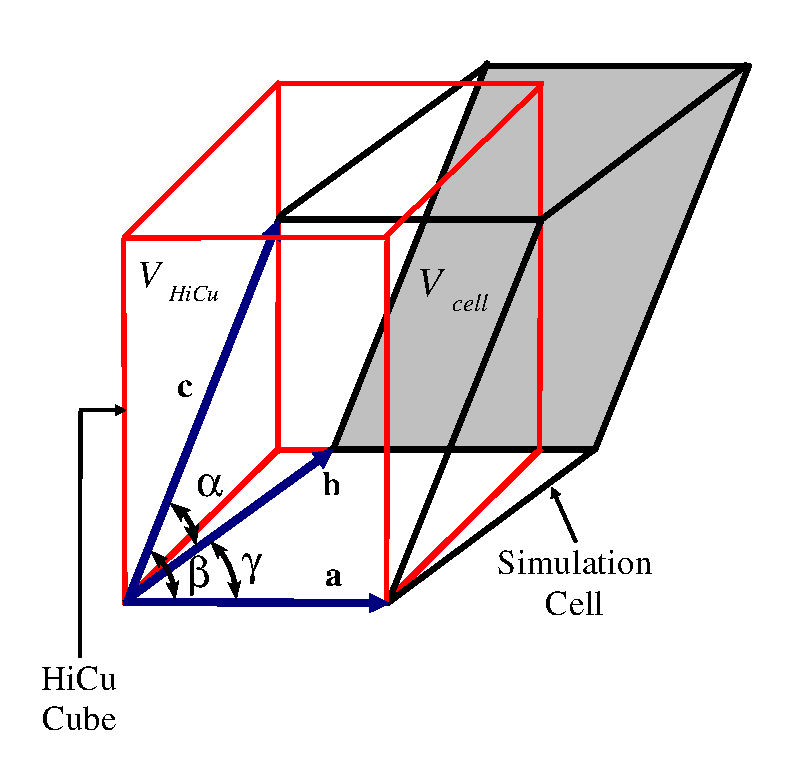
\includegraphics{UnitCell.eps} \par}
\end{figure}

\begin{figure}

\caption{\label{figure: ReplicateCells} Regions which contribute to the Coulomb Matrix}

{\par\centering 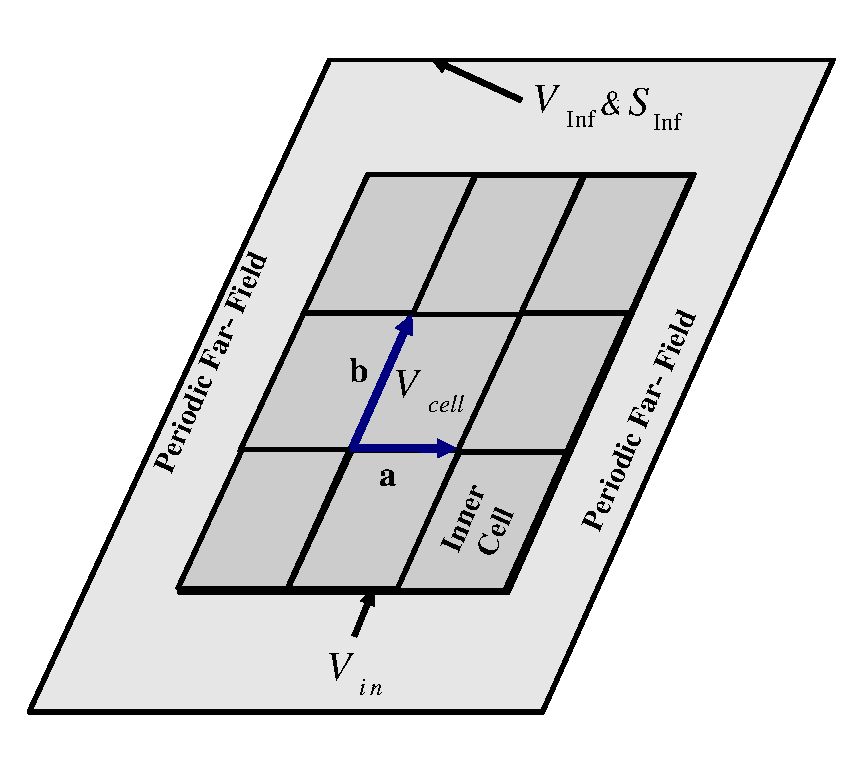
\includegraphics{RepCell.eps} \par}
\end{figure}



\begin{figure}

\caption{\label{figure: ErrorPFF}Error in the Periodic Far Field Approximation with
increasing inner box size}

{\par\centering \resizebox*{1.1\textwidth}{!}{\includegraphics{ErrorPFF_InnerBox.eps}} \par}
\end{figure}

\begin{figure}

\caption{\label{figure:DenseNitrogen} Iso-surface potential of a 100 molecule Dense
Nitrogen system}

{\par\centering \resizebox*{0.8\textwidth}{0.5\textheight}{\includegraphics{N2.eps}} \par}
\end{figure}

\begin{figure}

\caption{\label{figure: Scaling_Matrix_Build} Scaling Results for the matrix builds
\protect\( J_{QCTC}\protect \) and \protect\( K_{xc}\protect \) for the dense
molecular nitrogen periodic system.}
\end{figure}

\begin{figure}

\caption{\label{figure:Scaling_Diag} Scaling results for the overlap matrix inverter
and the density matrix solver. }
\end{figure}

\begin{figure}

\caption{\label{figure: Iso_zeolite} Iso-surface plot of zeolite.}
\end{figure}



\end{document}
